\section{Elementary Field Theory}

\begin{exercise}
\begin{figure}[H]
\centering
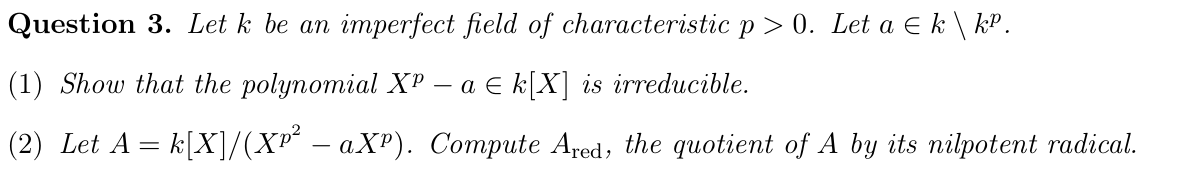
\includegraphics[width=\textwidth]{group-representation-2025050911.png}
% \caption{}
\label{}
\end{figure}
\end{exercise}
A \textbf{perfect field} $K$ can be characterized in several equivalent ways:

\begin{enumerate}
	\item Separable Extensions: Every algebraic extension of $K$ is a separable extension. (An algebraic extension is separable if the minimal polynomial of every element in the extension over $K$ has distinct roots.)
	\item Separable Polynomials: Every irreducible polynomial in $K[x]$ (the ring of polynomials with coefficients in $K$) is separable (has distinct roots in its splitting field).
	\item Characteristic Property:
	\begin{itemize}
		\item If $K$ has characteristic 0 (like $\mathbb{Q}, \mathbb{R}, \mathbb{C}$), it is always perfect.
		\item If $K$ has characteristic $p>0$ (where $p$ is a prime number), then $K$ is perfect if and only if the Frobenius endomorphism $F: K \rightarrow K$, defined by $F(a)=a^p$ for all $a \in K$, is surjective. This means that every element in $K$ is a $p$-th power of some element in $K$ (i.e., $K^p=K$). Since the Frobenius endomorphism is always injective for fields, this condition means it must be an automorphism.
	\end{itemize}
\end{enumerate}

\textbf{Examples of perfect fields} include:

\begin{itemize}
	\item All fields of characteristic 0 (e.g., the rational numbers $\mathbb{Q}$, the real numbers $\mathbb{R}$, the complex numbers $\mathbb{C}$).
	\item All finite fields (e.g., $\mathbb{F}_p=\mathbb{Z} / p \mathbb{Z}$ for a prime $p$, or $\mathbb{F}_{p^n}$). In finite fields, any injective map from the field to itself must also be surjective.
	\item All algebraically closed fields.
\end{itemize}

Now, an \textbf{imperfect field} is a field that does not satisfy these conditions. Based on the above:

\begin{itemize}
	\item An imperfect field must have characteristic $p>0$ for some prime $p$.
	\item In an imperfect field $K$ of characteristic $p>0$, the Frobenius endomorphism $a \mapsto a^p$ is not surjective. This means there exists at least one element in $K$ that cannot be written as the $p$-th power of any element in $K$ (i.e., $K^p \neq K$).
	\item Imperfect fields have at least one irreducible polynomial that is inseparable (i.e., has multiple roots in an extension field).
	\item There exist algebraic extensions of an imperfect field that are not separable.
\end{itemize}
